\documentclass[aspectratio=169]{beamer}
\usepackage{lmodern}
\usetheme{Madrid}
%\usecolortheme{giantoak}
\newcommand*\oldmacro{}
\let\oldmacro\insertshorttitle
\renewcommand*\insertshorttitle{\oldmacro\hfill\insertframenumber\,/\,\inserttotalframenumber}
\usepackage[framemethod=tikz]{mdframed}

\usepackage{beamerthemesplit}
\usepackage{textpos}
\usepackage{pgf}
%\logo{\pgfputat{\pgfxy(0,-.4)}{\pgfbox[right,base]{\includegraphics[height=1.0cm]{logo.jpg}}}}
%\newcommand{\nologo}{\setbeamertemplate{logo}{}}
\usepackage{booktabs}
\usepackage{graphicx}
\theoremstyle{principle}
\newtheorem*{principle}{Design Principle}


\titlegraphic{\includegraphics[width=1.0\paperwidth]{cool-wind-800px.jpg}}

\title{Amendments}
%\author[Jeremy Kedziora]{Wind Data Science Team\\
%\small{Uptake}}
\date{}

\begin{document}

%{
%%\nologo
%\begin{frame}
%    \maketitle
%\end{frame}
%}
%pages 1-7, 8-9, 14-15.


{
  \usebackgroundtemplate{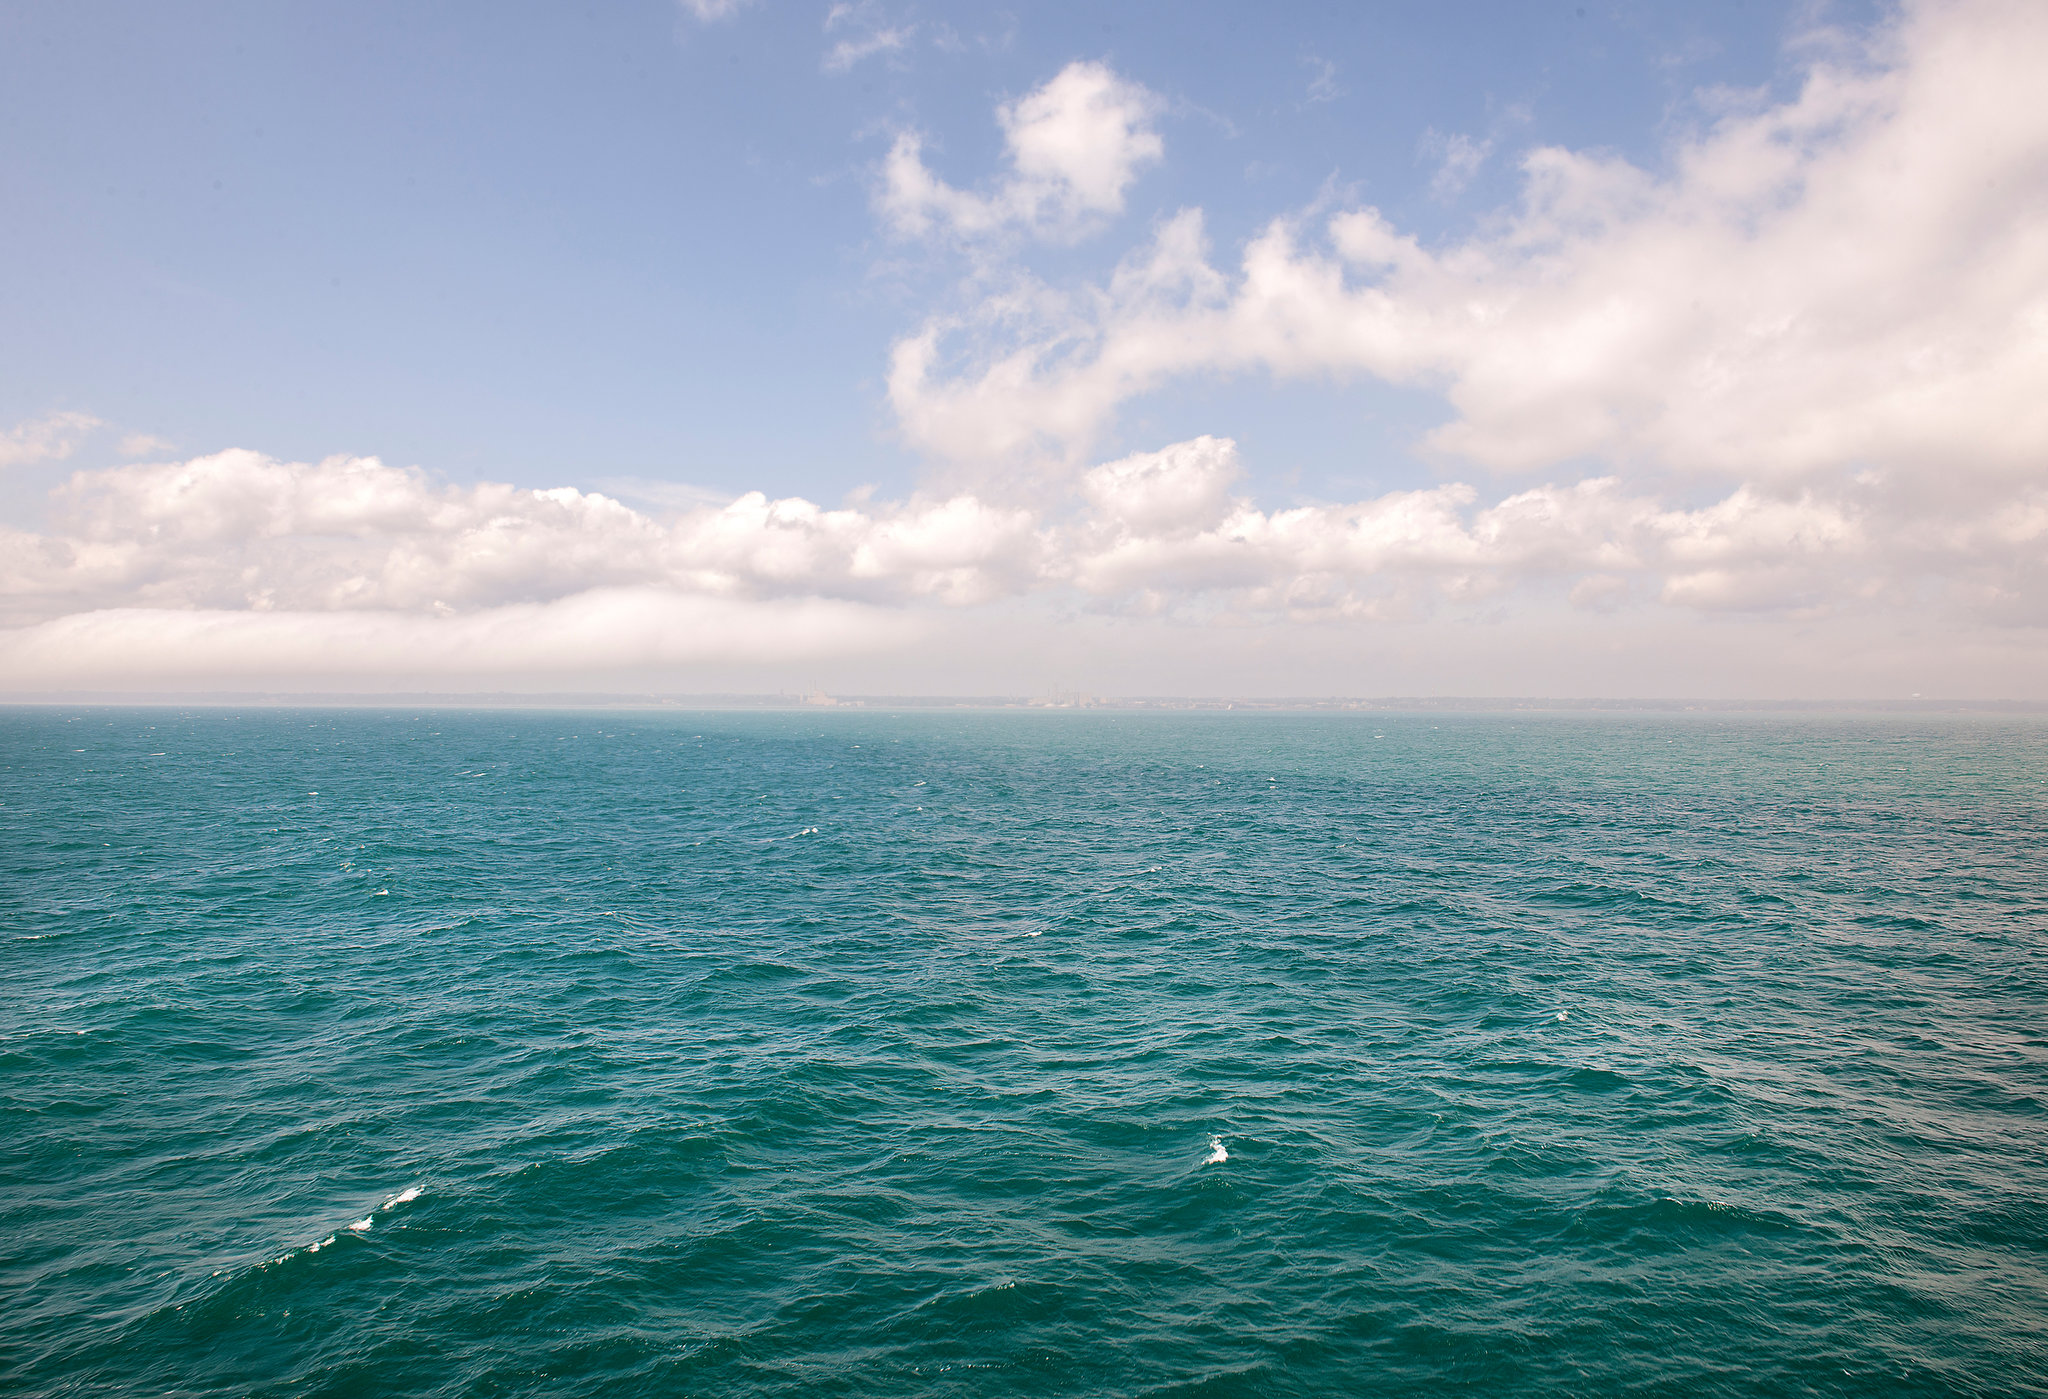
\includegraphics[width=1.0\paperwidth]{lake_michigan.jpg}}
  \begin{frame}[plain]
  
\begin{mdframed}[tikzsetting={draw=black,fill=white,fill opacity=0.7,
               line width=0pt},backgroundcolor=none,leftmargin=20,
               rightmargin=20,innertopmargin=4pt]
\Huge The Death and Life of the Great Lakes
\end{mdframed}

  \end{frame}
}

%@@@@@@@@@@@@@@@@@@@@@@@@@@@@@@@@@@@@@@@@@@@@@@@@@
%\begin{frame}
%
%\begin{center}
%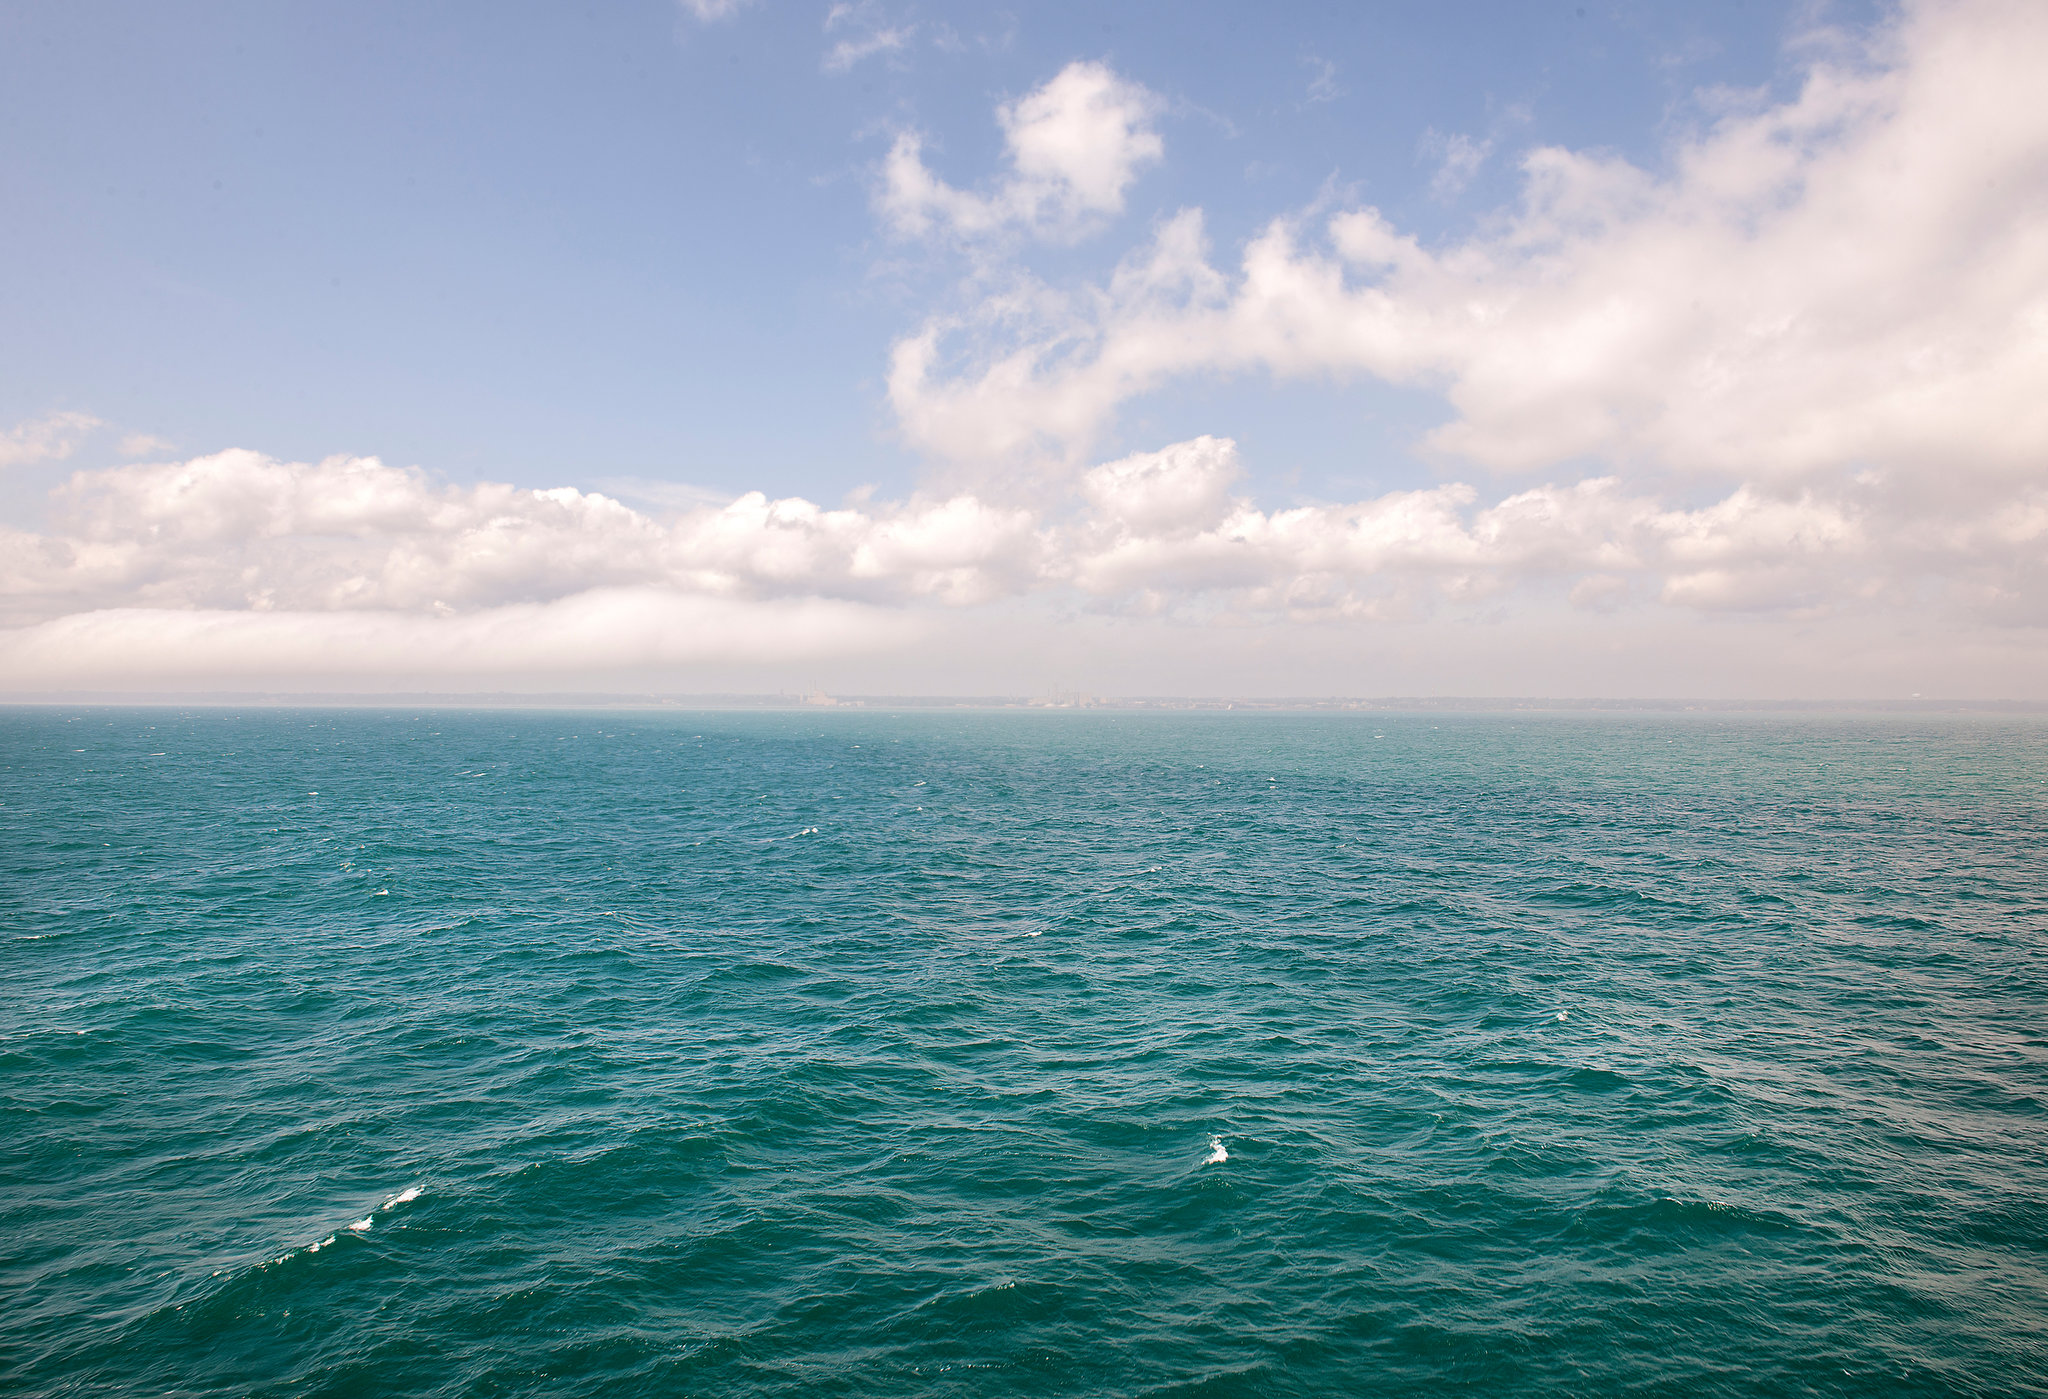
\includegraphics[scale=0.4]{lake_michigan.jpg}
%\end{center}
%
%
%\end{frame}

%@@@@@@@@@@@@@@@@@@@@@@@@@@@@@@@@@@@@@@@@@@@@@@@@@
\begin{frame}
\frametitle{The Death and Life of the Great Lakes Pt 1}

\begin{columns}

\begin{column}{0.5\textwidth}
TL;DR:
\bigskip
\begin{itemize}
\item Egan part 1 documents a series of policy choices;
\bigskip
\item Those policy choices induced successive waves of ecological instability in the Great Lakes system;
\end{itemize}

\end{column}

\onslide<1->
\begin{column}{0.5\textwidth}  %%<--- here
    \begin{center}
     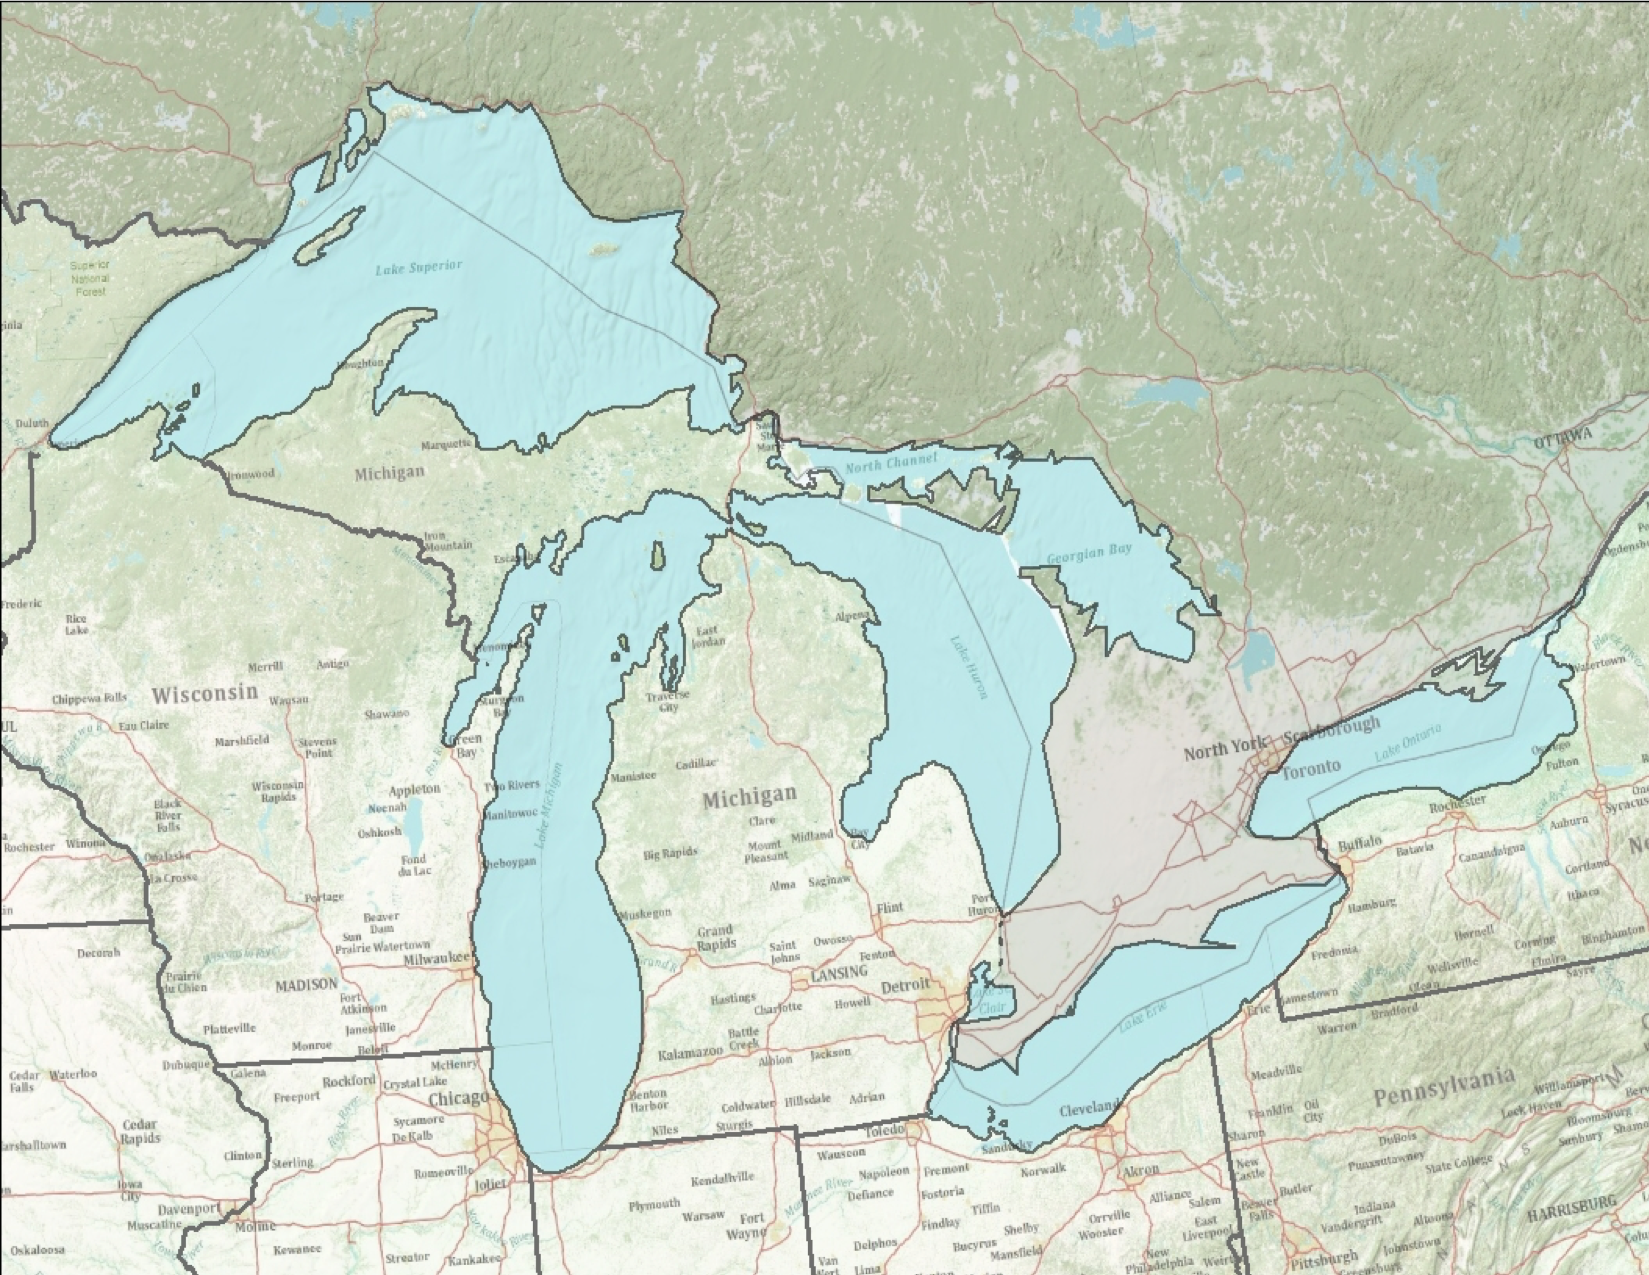
\includegraphics[scale=0.27]{great_lakes.png}
     \end{center}
\end{column}

\end{columns}

\end{frame}

%@@@@@@@@@@@@@@@@@@@@@@@@@@@@@@@@@@@@@@@@@@@@@@@@@
\begin{frame}
\frametitle{The Death and Life of the Great Lakes Pt 1}
We defined policy as a problem solving intent... so in these successive policies...
\begin{itemize}
\item What problems were they intended to solve?\onslide<2->
\bigskip
\bigskip
\item What actors were in a position to make choices and what were their authorities?\onslide<3->
\bigskip
\bigskip
\item What was in their evaluation criteria?\onslide<4->
\bigskip
\bigskip
\item What were the downstream consequences of their choices?\onslide<5->
\end{itemize}
\end{frame}

%@@@@@@@@@@@@@@@@@@@@@@@@@@@@@@@@@@@@@@@@@@@@@@@@@
\begin{frame}
\frametitle{Policy 1: canal building}
    \begin{center}
     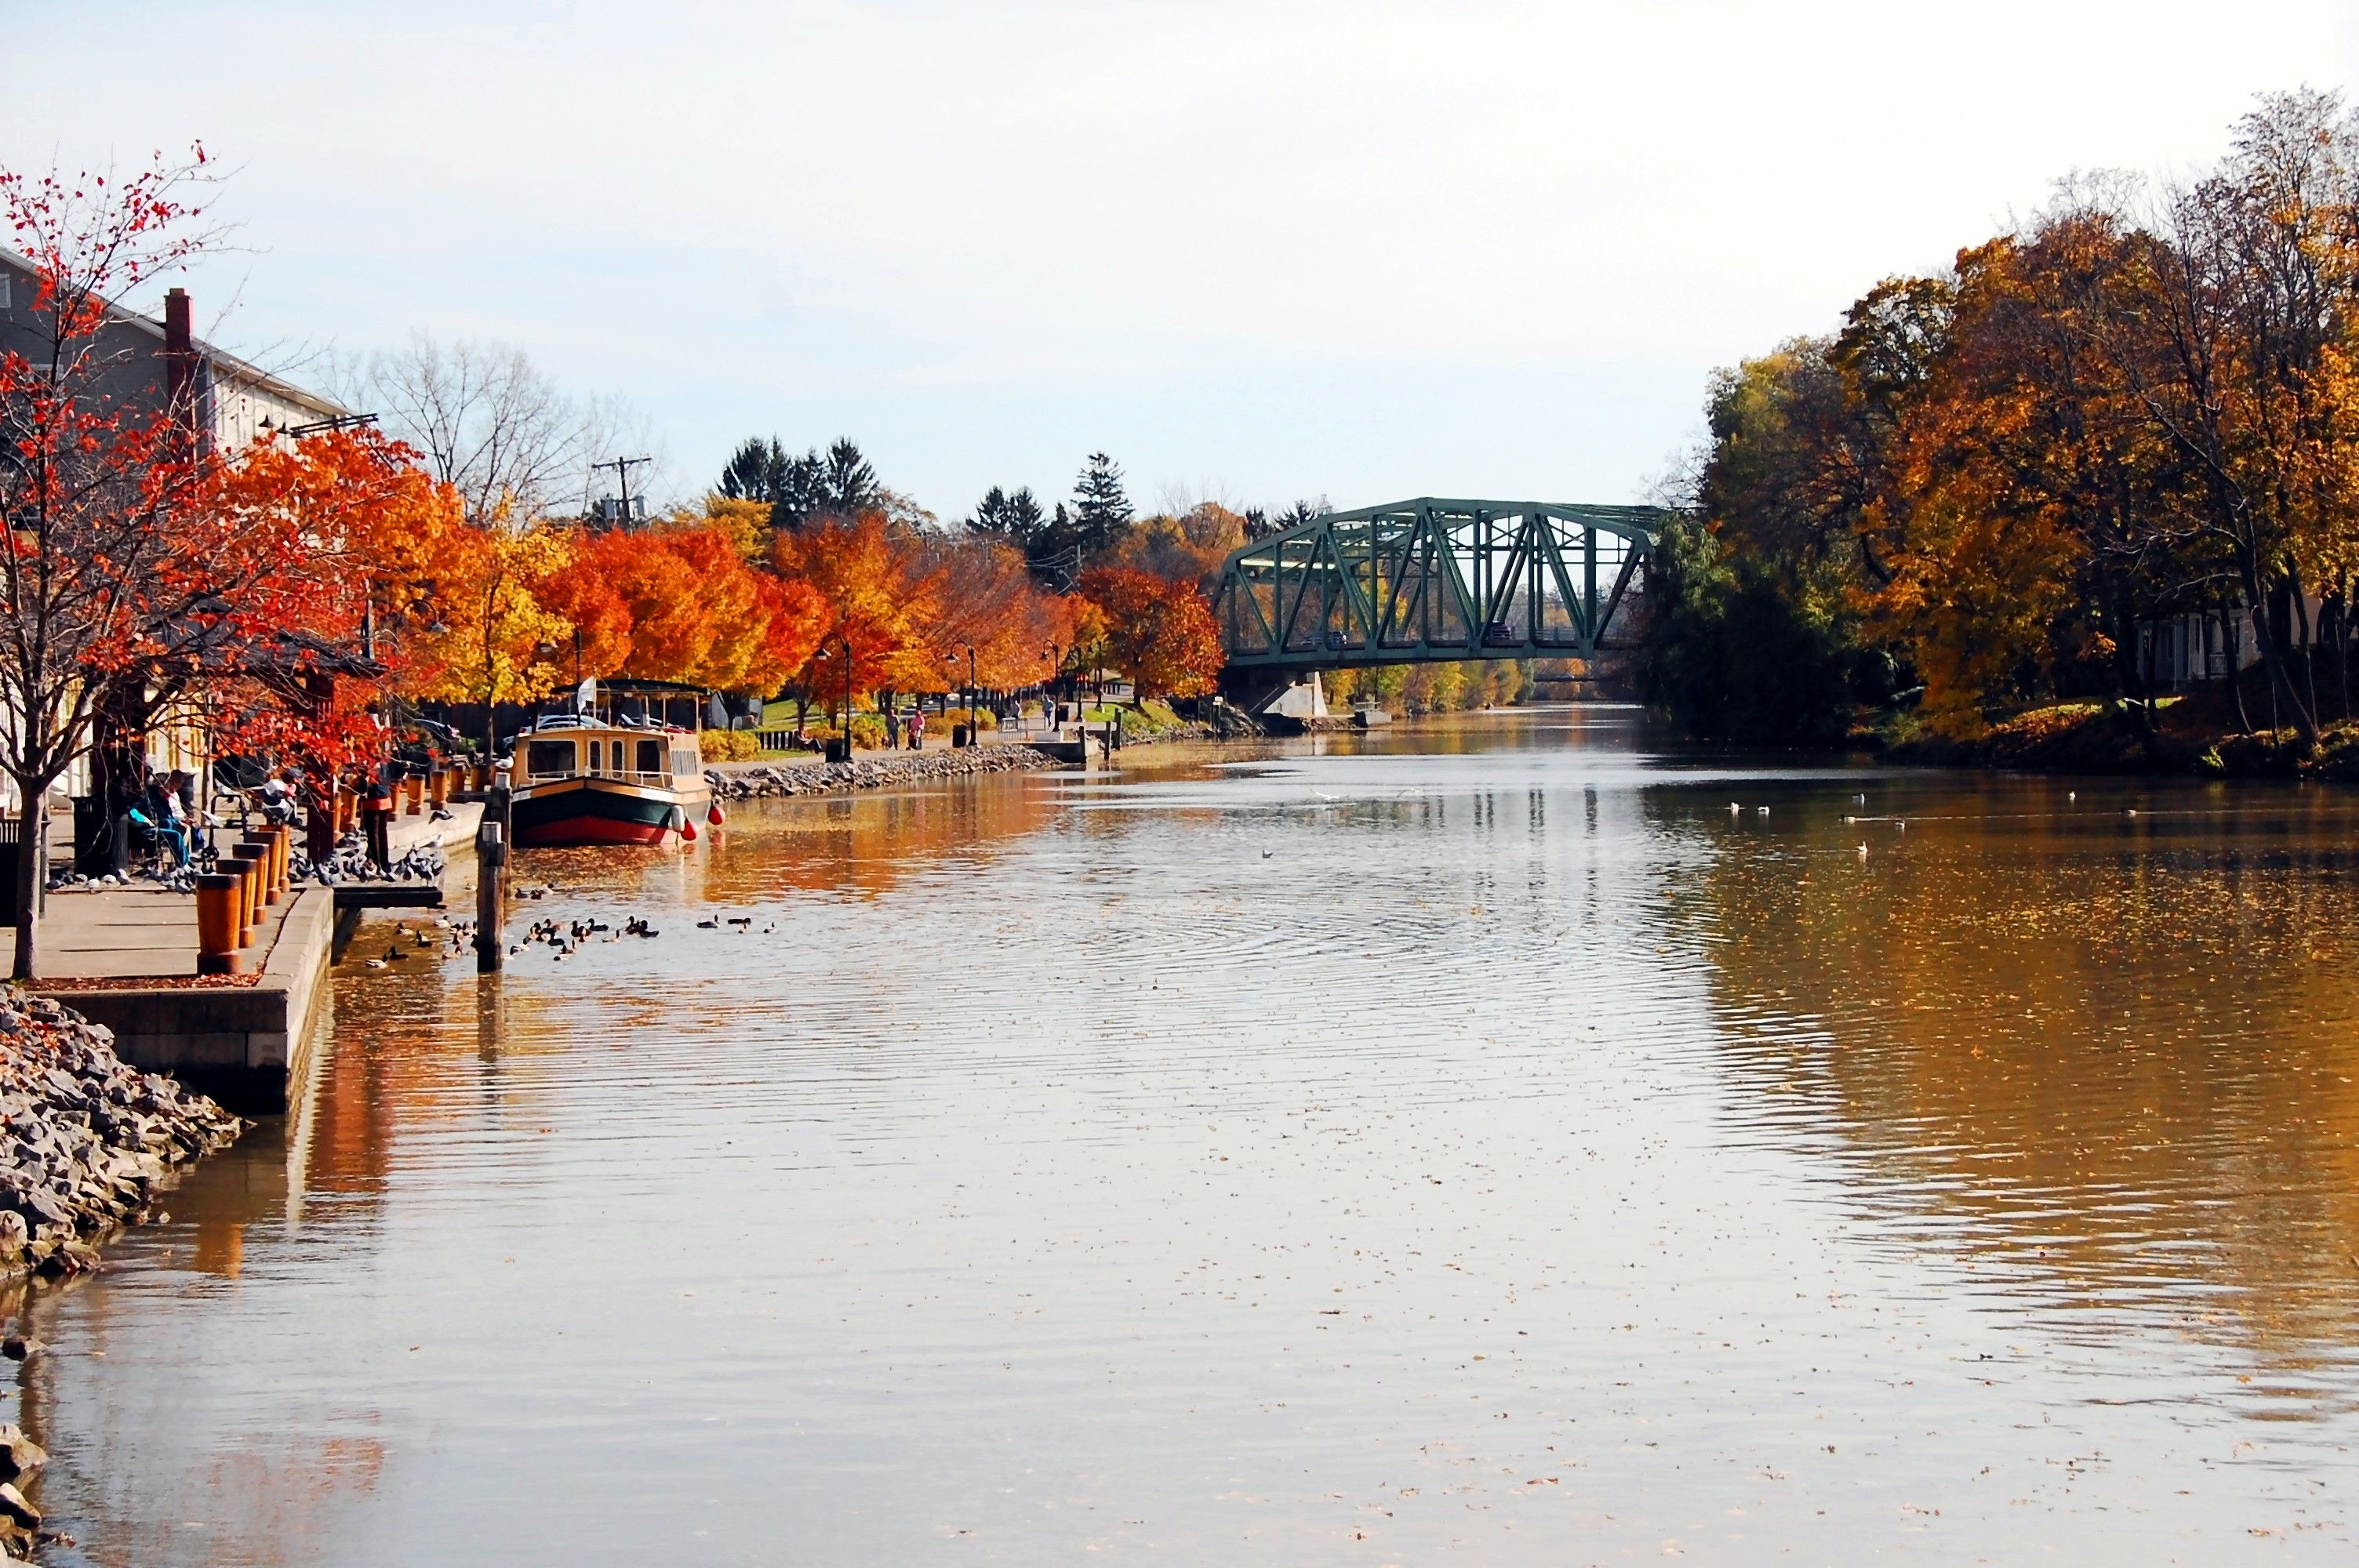
\includegraphics[scale=0.1]{erie_canal.jpg}
     \end{center}
%canal building
\end{frame}

%@@@@@@@@@@@@@@@@@@@@@@@@@@@@@@@@@@@@@@@@@@@@@@@@@
\begin{frame}
\frametitle{Policy 1: canal building}
    \begin{center}
     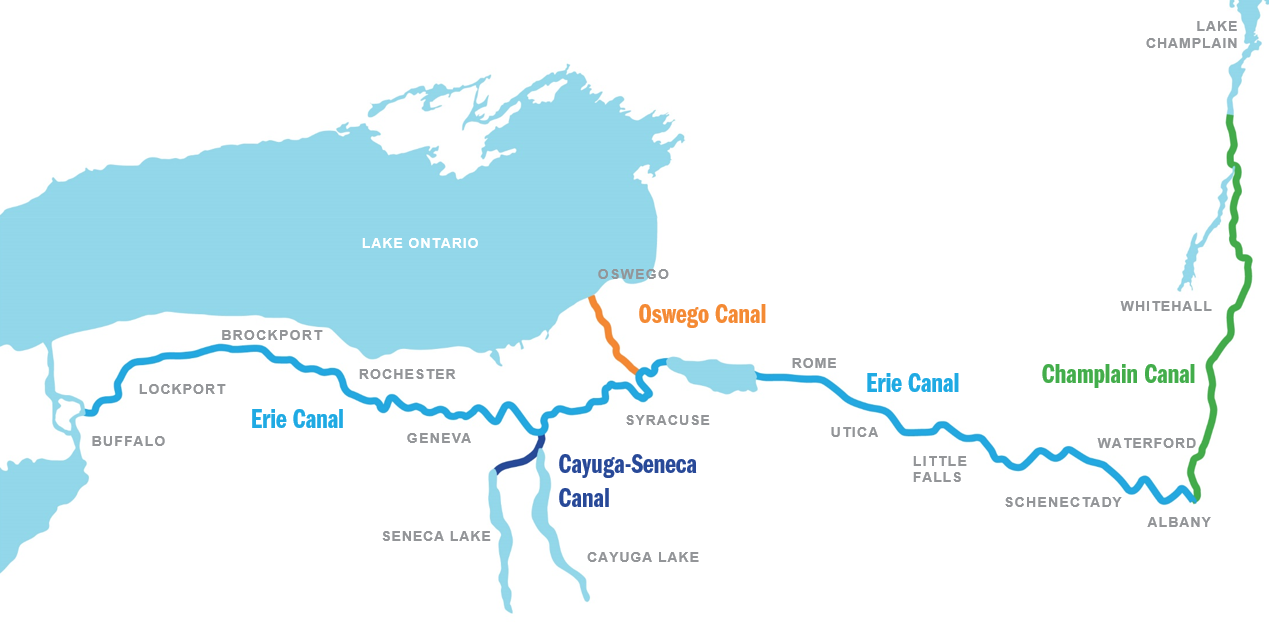
\includegraphics[scale=0.4]{erie_canal_map.png}
     \end{center}
%canal building
\end{frame}

%@@@@@@@@@@@@@@@@@@@@@@@@@@@@@@@@@@@@@@@@@@@@@@@@@
\begin{frame}
\frametitle{Policy 1: canal building}
    \begin{center}
     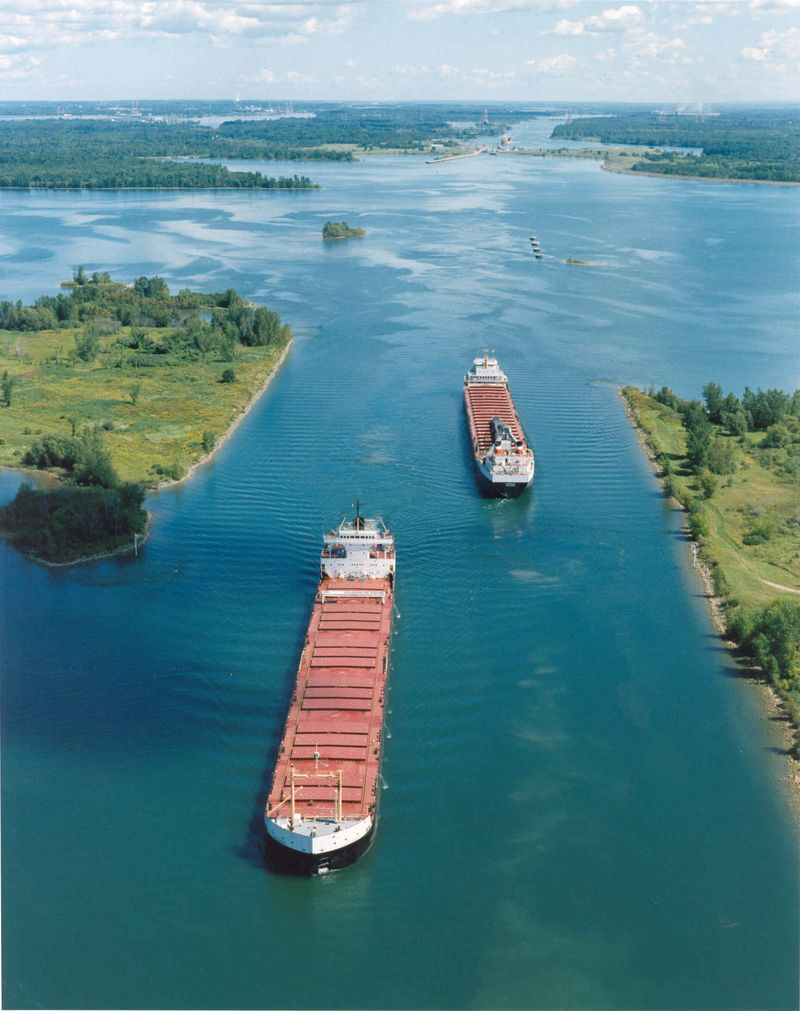
\includegraphics[scale=0.8]{st_lawrence_seaway.jpeg}
          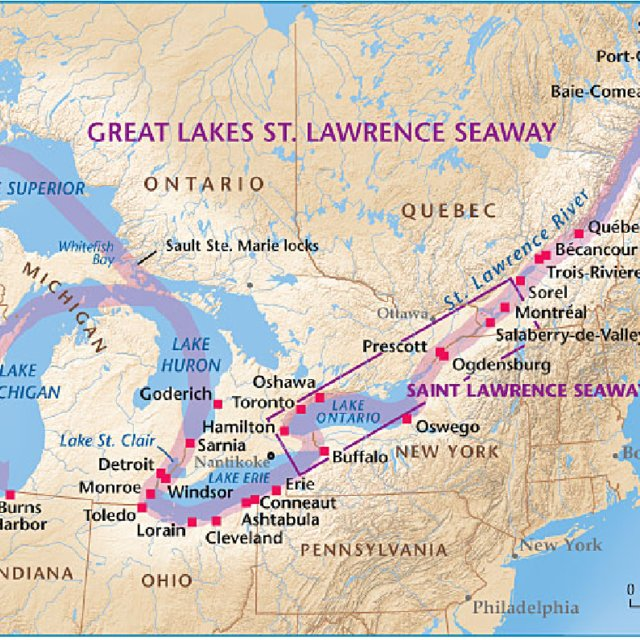
\includegraphics[scale=0.9]{st_lawrence_seaway_map.jpg}
     \end{center}
%canal building
\end{frame}

%@@@@@@@@@@@@@@@@@@@@@@@@@@@@@@@@@@@@@@@@@@@@@@@@@
\begin{frame}
\frametitle{Policy 1: canal building}

\begin{itemize}
\item Problem: 
\bigskip
\bigskip
\item Actors: 
\bigskip
\bigskip
\item Evaluation criteria: 
\bigskip
\bigskip
\item Policy: 
\bigskip
\bigskip
\item Consequences: 
\end{itemize}

\end{frame}

%@@@@@@@@@@@@@@@@@@@@@@@@@@@@@@@@@@@@@@@@@@@@@@@@@
\begin{frame}
\frametitle{Policy 1: canal building}

\begin{itemize}
\item Problem: Great Lakes unconnected to oceans by navigable water; others?
\bigskip
\bigskip
\item Actors: British army; DeWitt Clinton; Canada/Britain; Congress/Eisenhower; others?
\bigskip
\bigskip
\item Evaluation criteria: economic growth/development via trade;
\bigskip
\bigskip
\item Policy: build canals!  Welland, Erie, Seaway;
\bigskip
\bigskip
\item Consequences: ...
\end{itemize}

\end{frame}

%@@@@@@@@@@@@@@@@@@@@@@@@@@@@@@@@@@@@@@@@@@@@@@@@@
\begin{frame}
\frametitle{Policy 2: dealing with the first invasion}

    \begin{center}
     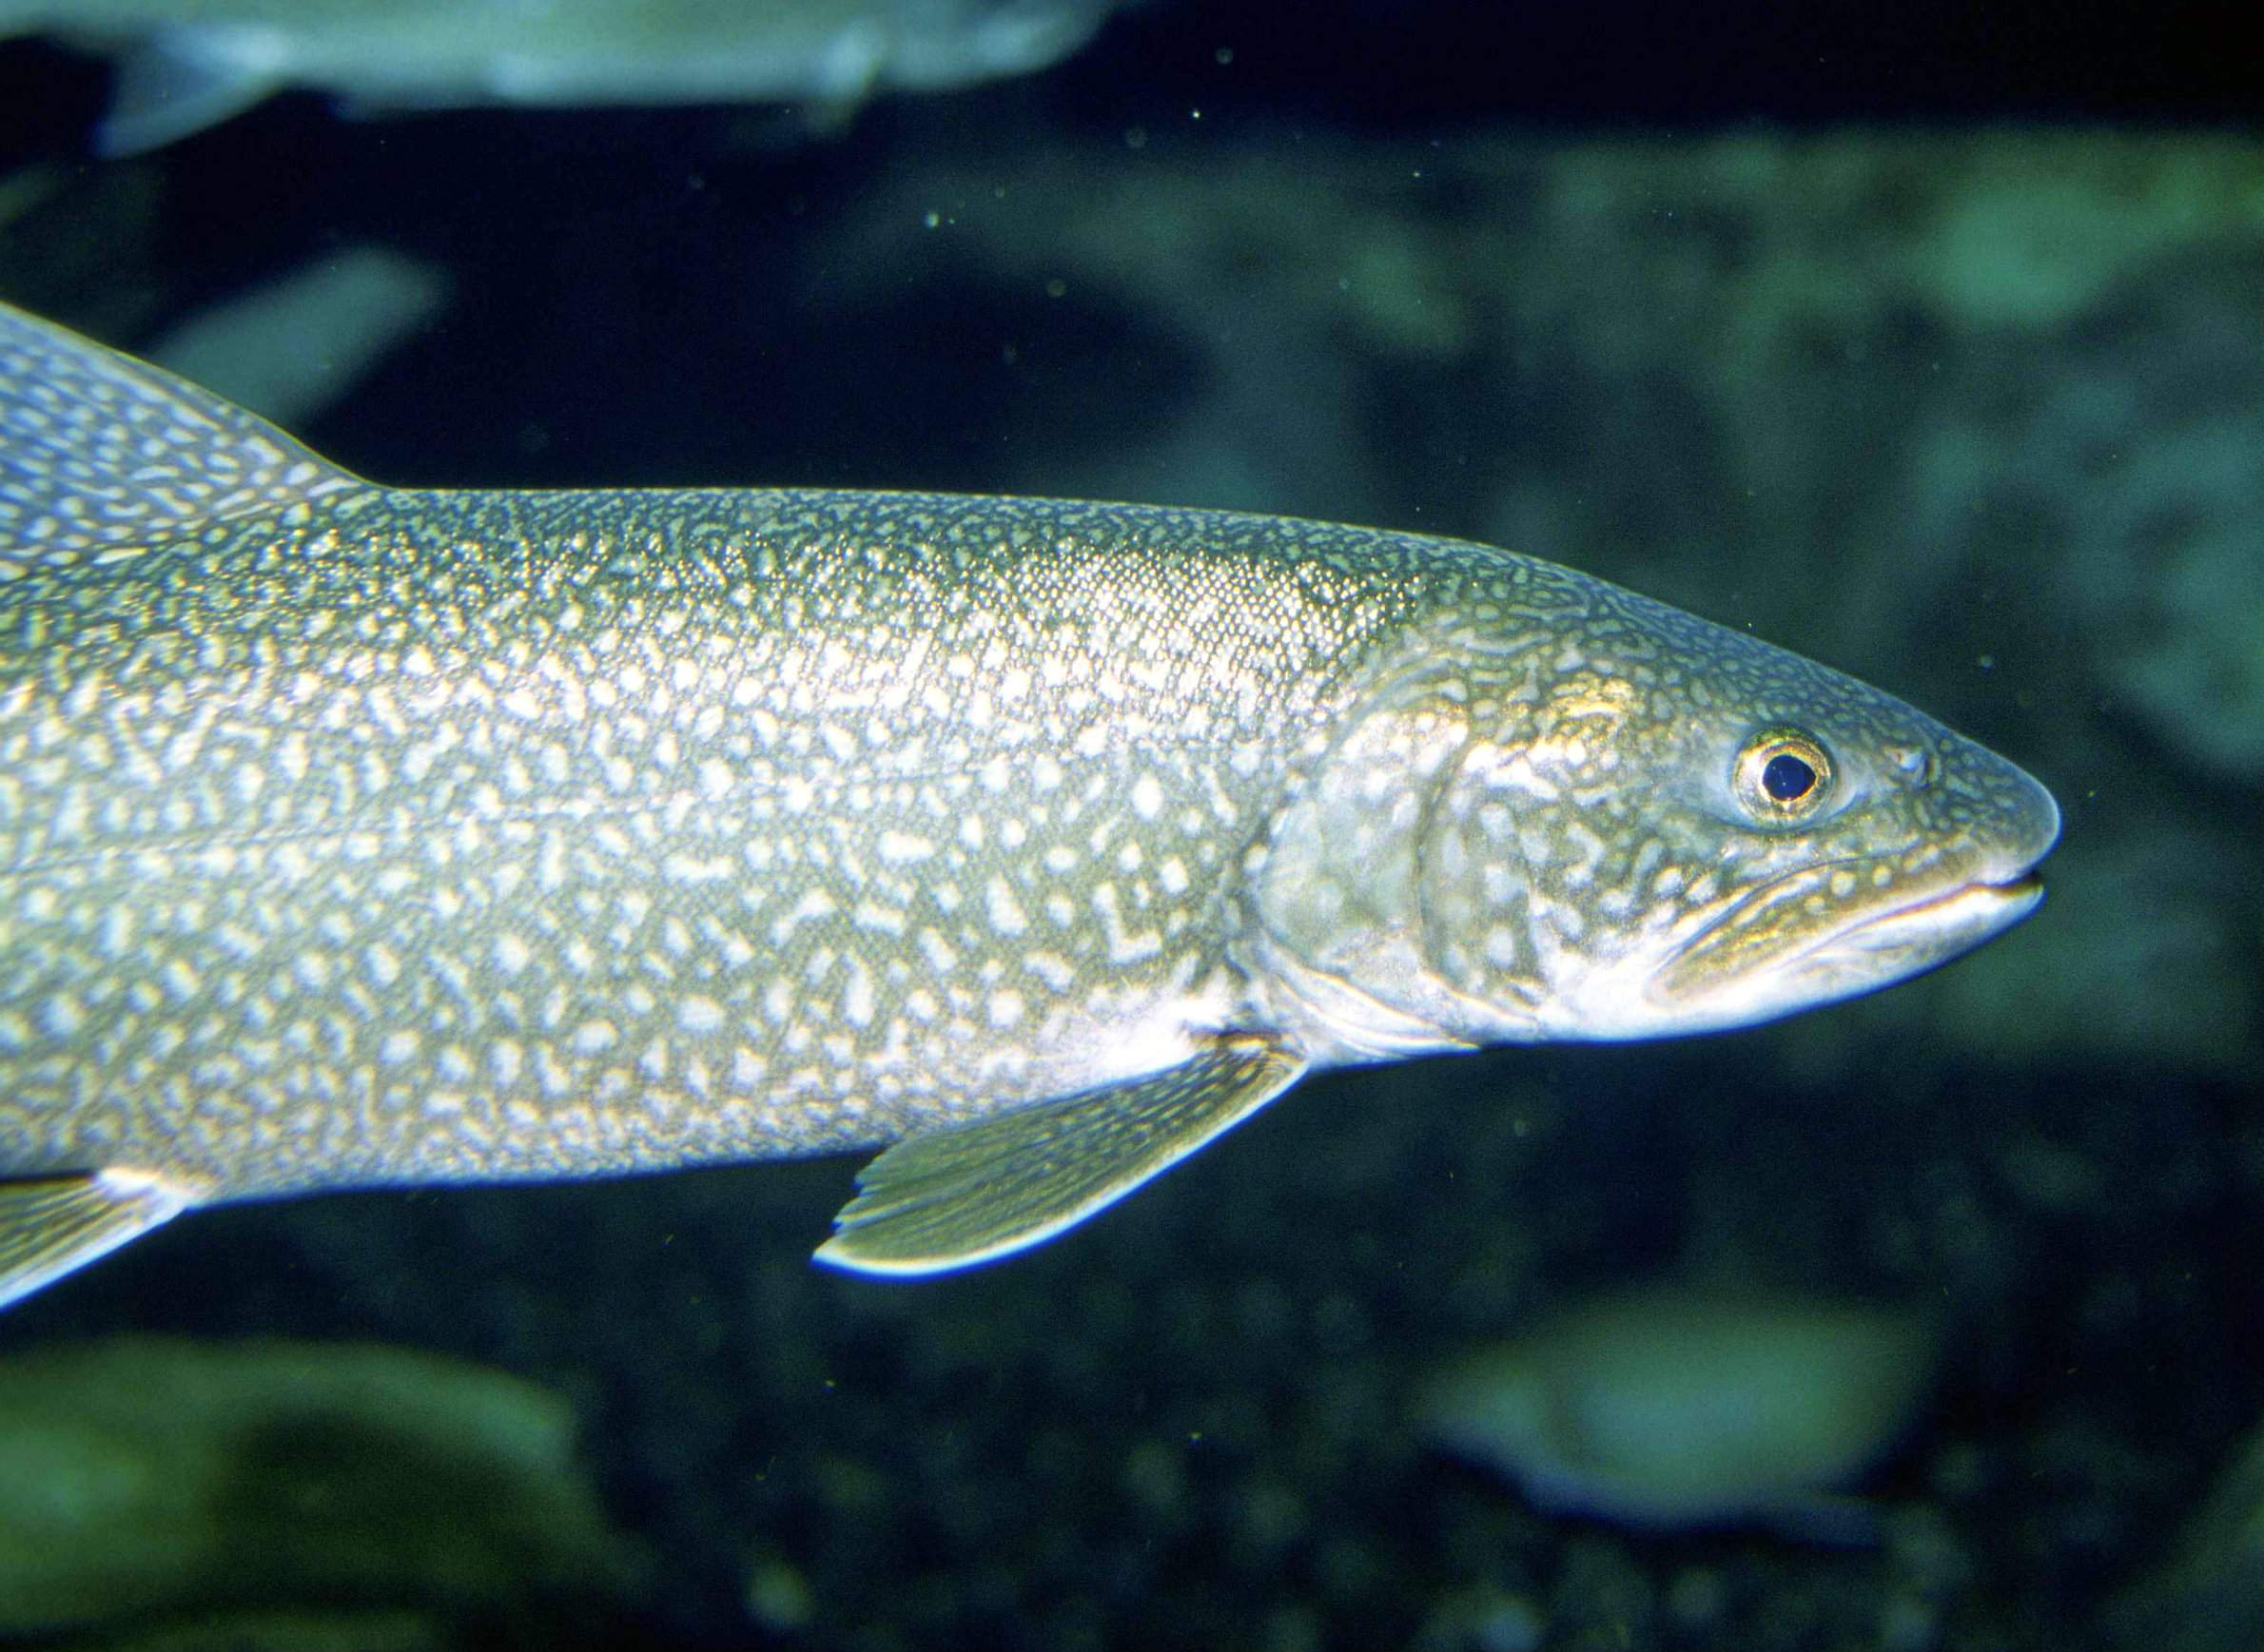
\includegraphics[scale=0.087]{lake_trout.jpg}
          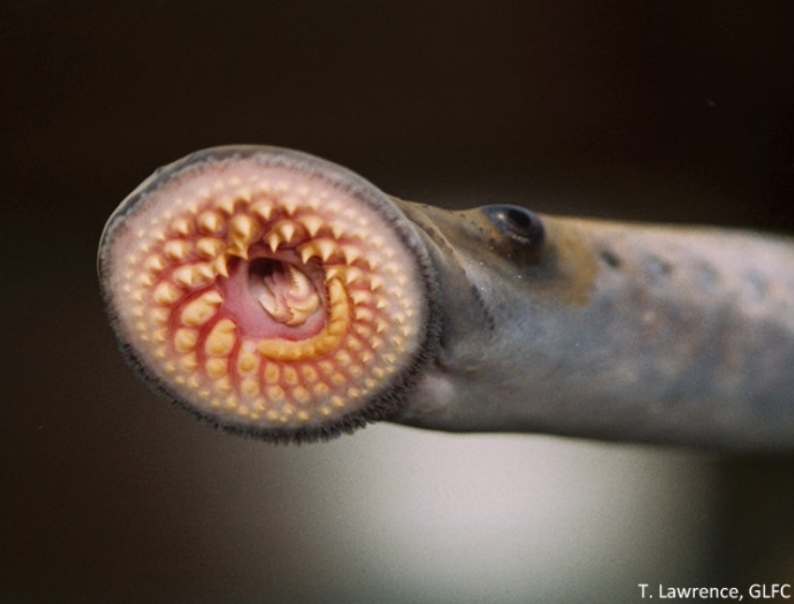
\includegraphics[scale=0.5]{sea_lamprey.png}
     \end{center}

\end{frame}

%@@@@@@@@@@@@@@@@@@@@@@@@@@@@@@@@@@@@@@@@@@@@@@@@@
\begin{frame}
\frametitle{Policy 2: dealing with the first invasion}

\begin{itemize}
\item Sea lamprey discovered in Lake Ontario in 1835 - may have swum through the Erie canal;
\bigskip
\bigskip
\item Found above Niagara Falls in Lake Erie in 1921;
\bigskip
\bigskip
\item Lake Michigan in 1936;
\bigskip
\bigskip
\item Lake Michigan lake trout harvest 6.5 million pounds in 1944 - only 324k pounds in 1949.
\end{itemize}

\end{frame}

%@@@@@@@@@@@@@@@@@@@@@@@@@@@@@@@@@@@@@@@@@@@@@@@@@
\begin{frame}
\frametitle{Policy 2: dealing with the first invasion}

\begin{itemize}
\item Problem: 
\bigskip
\bigskip
\item Actors: 
\bigskip
\bigskip
\item Evaluation criteria: 
\bigskip
\bigskip
\item Policy:
\bigskip
\bigskip
\item Consequences: 
\end{itemize}

\end{frame}

%@@@@@@@@@@@@@@@@@@@@@@@@@@@@@@@@@@@@@@@@@@@@@@@@@
\begin{frame}
\frametitle{Policy 2: dealing with the first invasion}

\begin{itemize}
\item Problem: collapse of native top of the food chain decimated commercial fishing;
\bigskip
\bigskip
\item Actors: US Fish and Wildlife Service; Applegate;
\bigskip
\bigskip
\item Evaluation criteria: restore the Great Lakes' natural apex predators; maintain canal links;
\bigskip
\bigskip
\item Policy: poison spawning grounds;
\bigskip
\bigskip
\item Consequences: Lamprey population $<$ 10\% of peak by 1967 -- too late for lake trout.
\end{itemize}

\end{frame}

%@@@@@@@@@@@@@@@@@@@@@@@@@@@@@@@@@@@@@@@@@@@@@@@@@
\begin{frame}
\frametitle{Policy 3: dealing with the second invasion}

    \begin{center}
     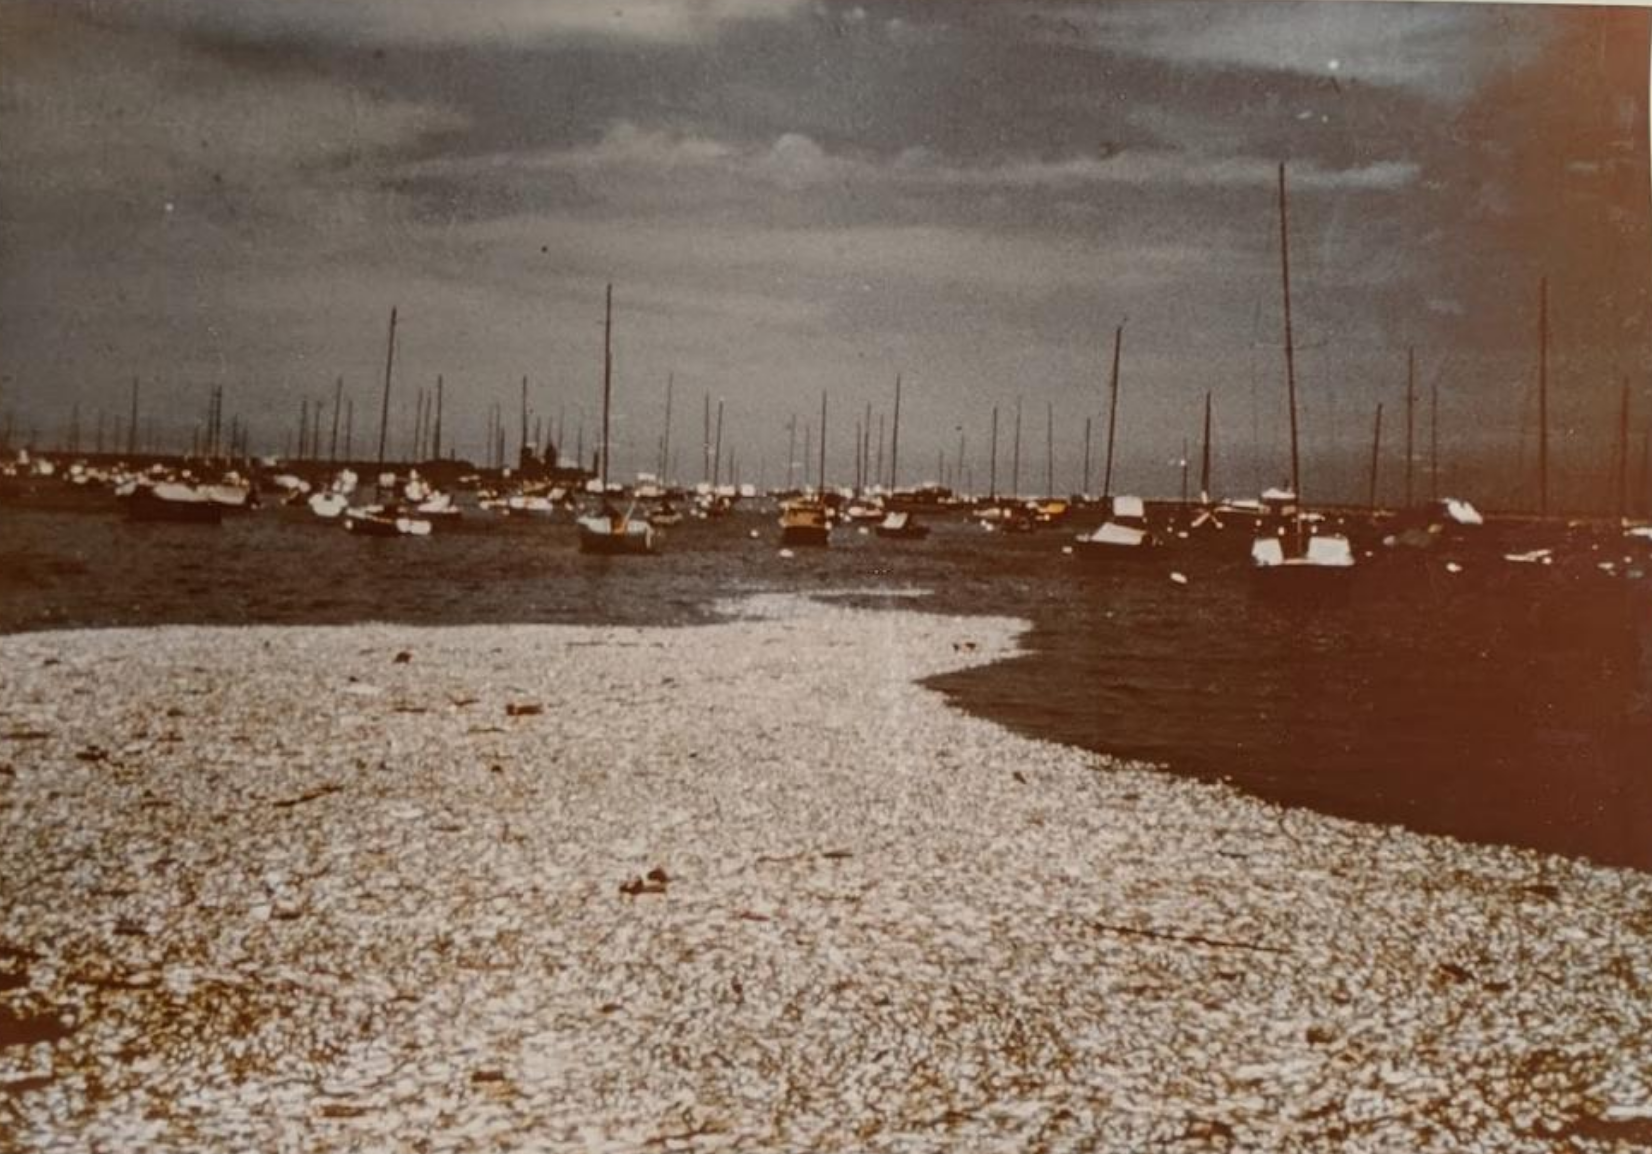
\includegraphics[scale=0.35]{chicago_alewife.png}
     \end{center}

\end{frame}

%@@@@@@@@@@@@@@@@@@@@@@@@@@@@@@@@@@@@@@@@@@@@@@@@@
\begin{frame}
\frametitle{Policy 3: dealing with the second invasion}

\begin{itemize}
\item Alewife (river herring) - an east coast fish and food source for more than 4k years, used as an early form of welfare in colonial America;
\bigskip
\bigskip
\item May be a natural addition to Lake Ontario - found there in 1873;
\bigskip
\bigskip
\item Overfishing decreased apex predator populations in Lake Ontario leading to Alewife population explosion;
\bigskip
\bigskip
\item Found in Lake Erie in 1931, in Lake Huron in 1933, in Lake Michigan in 1949, and in Lake Superior in 1954;
\bigskip
\bigskip
\item By 1965 they were 90\% of the fish mass in Lake Michigan; massive die-off.
\end{itemize}

\end{frame}

%@@@@@@@@@@@@@@@@@@@@@@@@@@@@@@@@@@@@@@@@@@@@@@@@@
\begin{frame}
\frametitle{Policy 3: dealing with the second invasion}

\begin{itemize}
\item Problem: 
\bigskip
\bigskip
\item Actors: 
\bigskip
\bigskip
\item Evaluation criteria: 
\bigskip
\bigskip
\item Policy: 
\bigskip
\bigskip
\item Consequences: 
\end{itemize}
\end{frame}

%@@@@@@@@@@@@@@@@@@@@@@@@@@@@@@@@@@@@@@@@@@@@@@@@@
\begin{frame}
\frametitle{Policy 3: dealing with the second invasion}

\begin{itemize}
\item Problem: commercial fishing destroyed; repeated massive die-offs decimated tourism; Lake Michigan biodiversity and ecological stability upset.
\bigskip
\bigskip
\item Actors: ``There are hundreds if not thousands of government bodies—from township boards to state environmental departments to Native American tribes to federal fishery agencies to the U.S. and Canadian International Joint Commission—that have some role in managing the interconnected lakes for the sake of the 50 million people who live within a short drive of their shores"; Michigan Fishery Chief Howard Tanner.
\bigskip
\bigskip
\item Evaluation criteria: ecological stability and fun; maintain canal links;
\bigskip
\bigskip
\item Policy: Import coho and chinook salmon into Lake Michigan; 
\bigskip
\bigskip
\item Consequences: explosion of recreational fishing, unsustainable salmon population growth. 
\end{itemize}

\end{frame}

%@@@@@@@@@@@@@@@@@@@@@@@@@@@@@@@@@@@@@@@@@@@@@@@@@
\begin{frame}
\frametitle{Policy 4: dealing with the third invasion}

    \begin{center}
     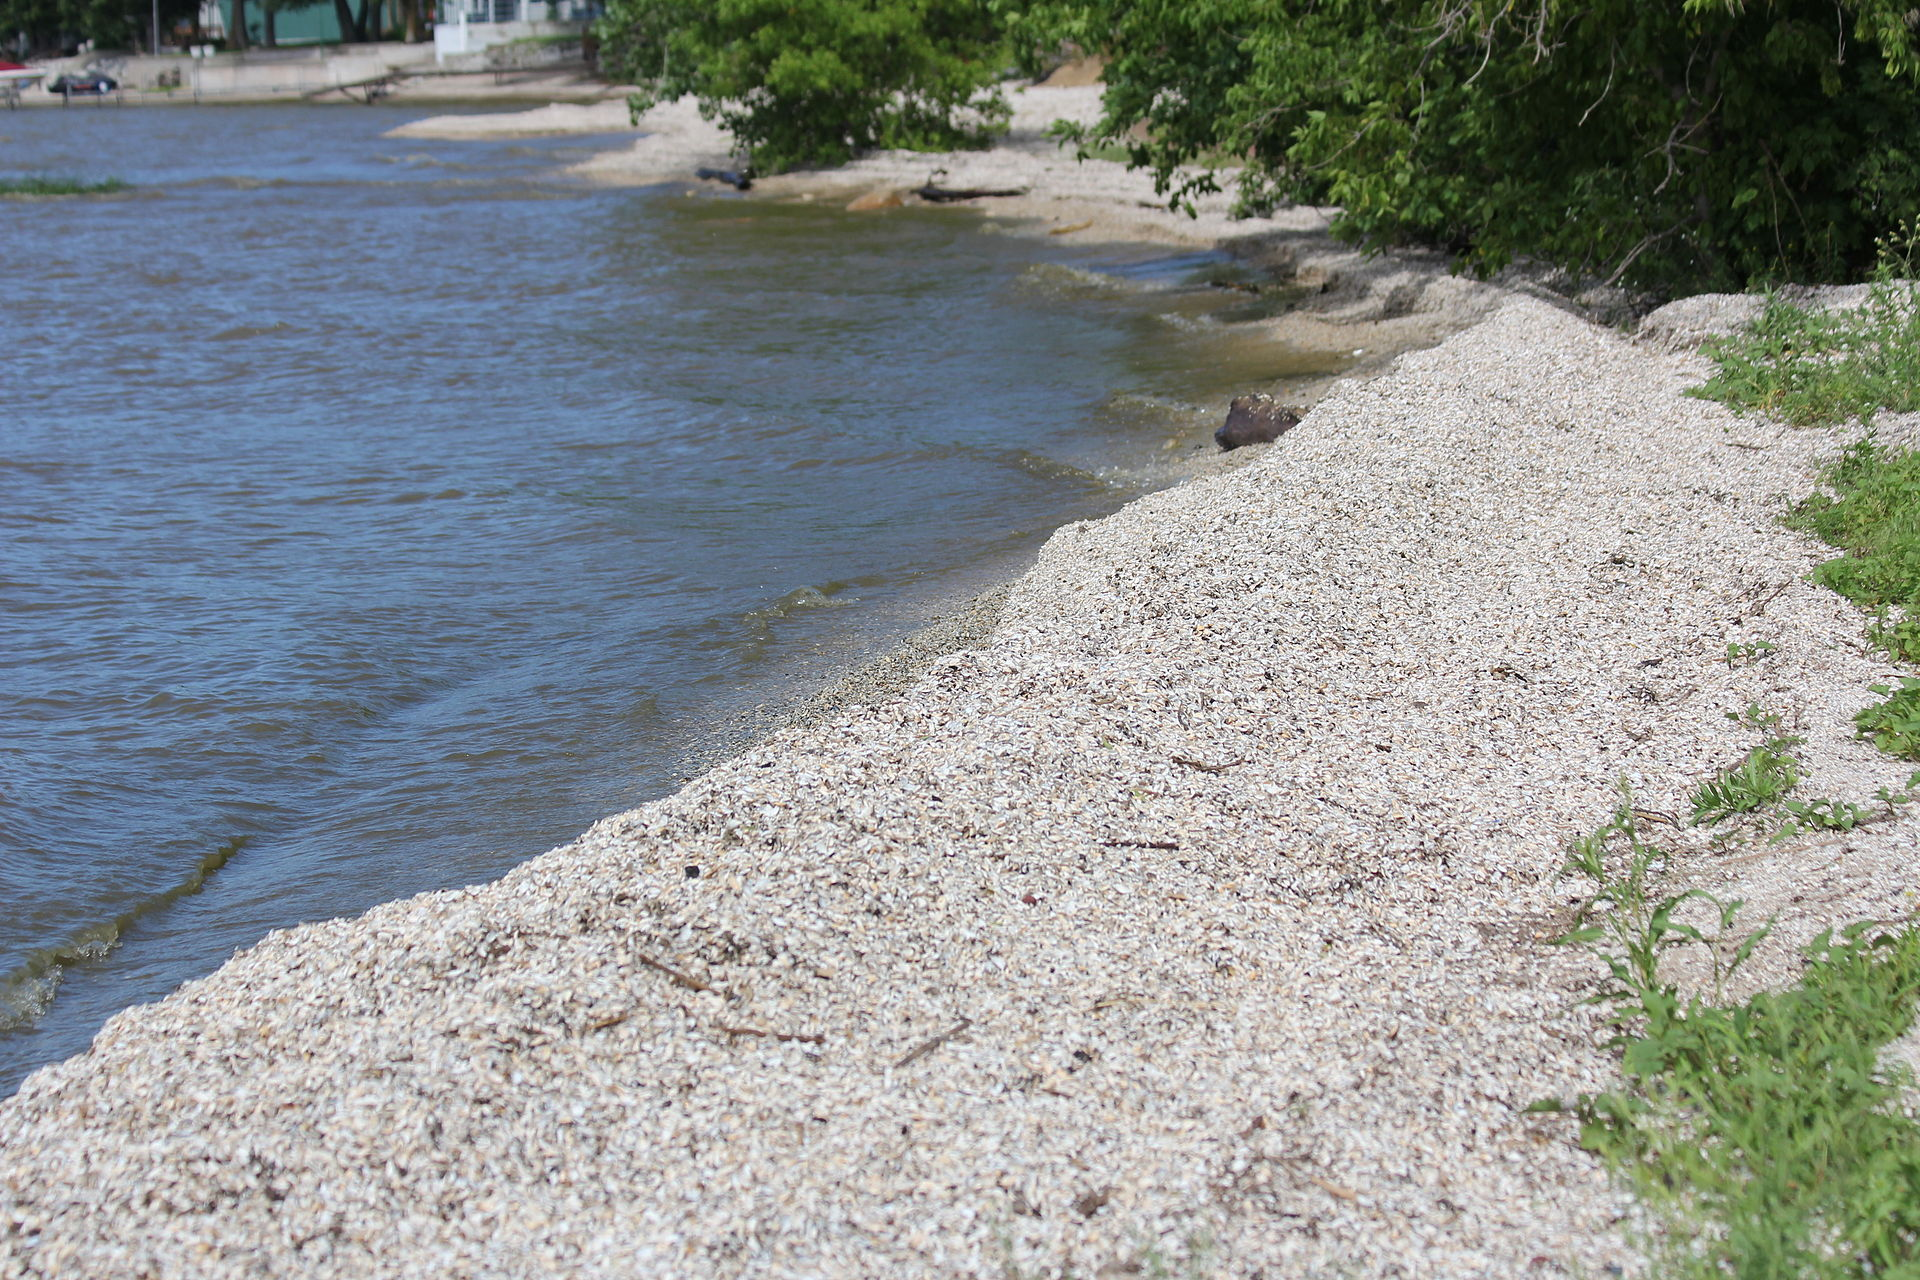
\includegraphics[scale=0.15]{zebra_mussels.jpg}
     \end{center}

\end{frame}

%@@@@@@@@@@@@@@@@@@@@@@@@@@@@@@@@@@@@@@@@@@@@@@@@@
\begin{frame}
\frametitle{Policy 4: dealing with the third invasion}

\begin{itemize}
\item With the opening of the seaway, exotic species quickly arrived in the Great Lakes;
\bigskip
\bigskip
\item First zebra mussel found in Lake St Claire in 1988;
\bigskip
\bigskip
\item Hypothesized to have arrived via water ballast from a ship;
\bigskip
\bigskip
\item Quagga mussel found in Lake Erie in 1989.
\end{itemize}

\end{frame}

%@@@@@@@@@@@@@@@@@@@@@@@@@@@@@@@@@@@@@@@@@@@@@@@@@
\begin{frame}
\frametitle{Policy 4: dealing with the third invasion}

    \begin{center}
    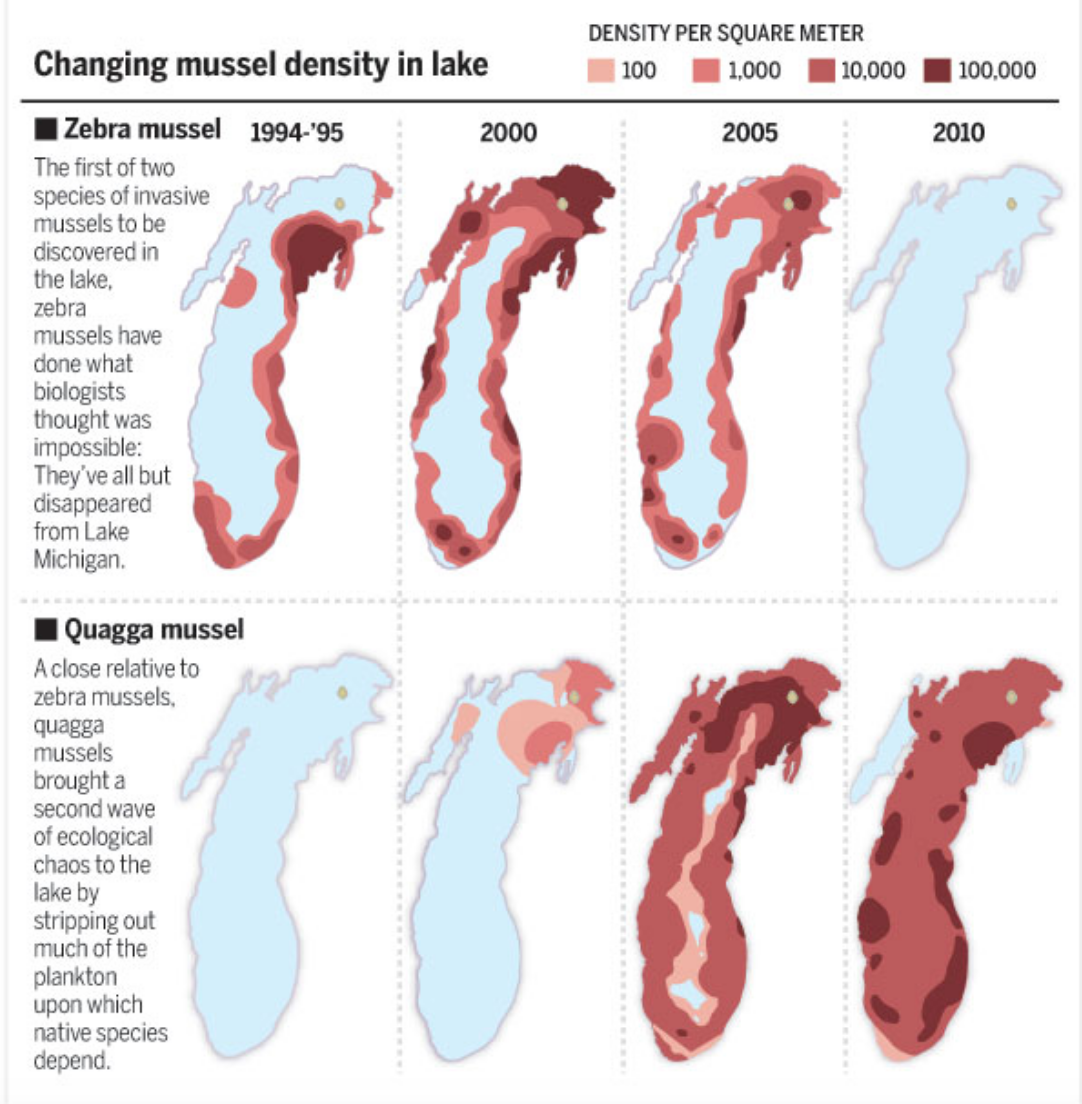
\includegraphics[scale=0.35]{quaggas_and_zebs.png}
     %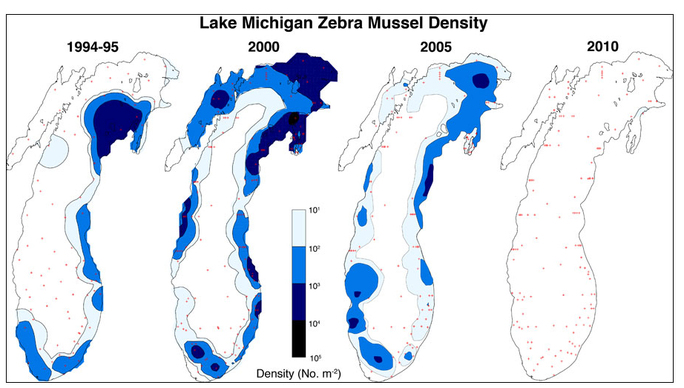
\includegraphics[scale=0.335]{zebra.jpg}
          %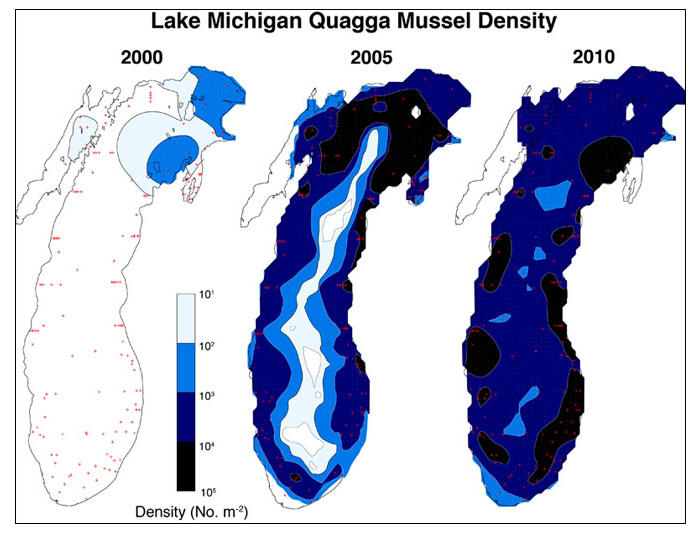
\includegraphics[scale=0.24]{quagga.jpg}
     \end{center}

\end{frame}

%@@@@@@@@@@@@@@@@@@@@@@@@@@@@@@@@@@@@@@@@@@@@@@@@@
\begin{frame}
\frametitle{Policy 4: dealing with the third invasion}

\begin{itemize}
\item Problem: 
\bigskip
\bigskip
\item Actors: 
\bigskip
\bigskip
\item Evaluation criteria: 
\bigskip
\bigskip
\item Policy: 
\bigskip
\bigskip
\item Consequences: 
\end{itemize}
\end{frame}

%@@@@@@@@@@@@@@@@@@@@@@@@@@@@@@@@@@@@@@@@@@@@@@@@@
\begin{frame}
\frametitle{Policy 4: dealing with the third invasion}

\begin{itemize}
\item Problem: destruction of the base of the food chain;
\bigskip
\bigskip
\item Actors: EPA; US coast guard; Isle Royale National Park Superintendent Phyllis Green;
\bigskip
\bigskip
\item Evaluation criteria: stop importing exotic species; maintain canal links;
\bigskip
\bigskip
\item Policy: mandatory ballast flushing before entering the Great Lakes; development of ballast treatment systems; 
\bigskip
\bigskip
\item Consequences: ???
\end{itemize}

\end{frame}

%%@@@@@@@@@@@@@@@@@@@@@@@@@@@@@@@@@@@@@@@@@@@@@@@@@
%\begin{frame}
%\frametitle{Policy 4: dealing with the third invasion}
%
%    \begin{center}
%    \includegraphics[scale=0.2,angle=270]{sk1.jpeg}
%        \includegraphics[scale=0.2,angle=270]{sk2.jpeg}
%     \end{center}
%
%
%\end{frame}
%
%
%%@@@@@@@@@@@@@@@@@@@@@@@@@@@@@@@@@@@@@@@@@@@@@@@@@
%\begin{frame}
%\frametitle{Final Thoughts}
%
%\begin{itemize}
%\item Do you buy Egan's `big person of history' story?
%\bigskip
%\bigskip
%\item What happens when more than one actor has authority to solve the problem?
%\bigskip
%\bigskip
%\item Arrow's Theorem: no ranked voting electoral system can convert individual ranked preferences into a community-wide ranking `rationally.'
%\bigskip
%\bigskip
%\item Median Voter Theorem: a majority rule voting system will select the outcome most preferred by the median voter.
%\end{itemize}
%
%\end{frame}



\end{document}








